\documentclass[11pt,a4paper]{article}
\usepackage[T1]{fontenc}
\usepackage[utf8]{inputenc}
\usepackage{lmodern}
\usepackage{microtype}
\usepackage[top=2.2cm,bottom=2.5cm,left=2.5cm,right=5.5cm,marginparwidth=4cm,marginparsep=0.5cm]{geometry}
\usepackage{setspace}\setstretch{1.15}
\usepackage[parfill]{parskip}
\usepackage[dvipsnames]{xcolor}
\definecolor{linkblue}{HTML}{1A5276}
\definecolor{accentteal}{HTML}{117864}
\definecolor{darkgray}{HTML}{2C3E50}
\definecolor{rulegray}{HTML}{BDC3C7}
\usepackage{marginnote}
\renewcommand*{\marginfont}{\footnotesize\sffamily}
\newcommand{\defn}[2][0pt]{\marginnote{\fcolorbox{accentteal!30}{accentteal!6}{\parbox{3.5cm}{\raggedright\footnotesize\sffamily\color{accentteal}\vspace{2pt}#2\vspace{2pt}}}}[#1]}
\usepackage{titlesec}
\titleformat{\section}{\Large\bfseries\color{darkgray}}{\thesection}{0.6em}{}
\titleformat{\subsection}{\large\bfseries\color{darkgray}}{\thesubsection}{0.5em}{}
\titlespacing*{\section}{0pt}{2em}{0.6em}
\titlespacing*{\subsection}{0pt}{1.2em}{0.4em}
\usepackage{fancyhdr}\pagestyle{fancy}\fancyhf{}
\fancyhead[L]{\small\color{gray}\textit{Barrantes --- Fraud prevention, ML, and design patterns}}
\fancyhead[R]{\small\color{gray}\textit{Nerdearla Chile 2026}}
\fancyfoot[C]{\small\thepage}
\renewcommand{\headrulewidth}{0.3pt}\renewcommand{\footrulewidth}{0pt}
\fancyhfoffset[R]{3.5cm}
\usepackage{graphicx}\graphicspath{{../../img/}}
\usepackage{float}
\usepackage[font=small,labelfont=bf,labelsep=period,justification=centering,margin=0.5cm]{caption}
\usepackage{enumitem}
\setlist[itemize]{nosep,left=0pt..1.5em}
\setlist[enumerate]{nosep,left=0pt..1.5em}
\usepackage{booktabs}
\usepackage[colorlinks=true,linkcolor=linkblue,citecolor=accentteal,urlcolor=linkblue,bookmarks=true,bookmarksnumbered=true,pdfauthor={José P. Barrantes},pdftitle={Designing fraud-prevention systems that keep analysts in the loop}]{hyperref}
\usepackage{url}\urlstyle{same}
\usepackage[round,sort&compress]{natbib}\bibliographystyle{apalike}

\begin{document}

\begin{center}
{\LARGE\bfseries Designing fraud-prevention systems\\[0.25em]that keep analysts in the loop\par}
\vspace{0.6em}
{\large José P.\ Barrantes\par}\vspace{0.3em}
{\normalsize IBM\enspace$\cdot$\enspace Programa de Posgrado en Computación e Informática, Universidad de Costa Rica\par}\vspace{0.2em}
{\small\href{mailto:jospablo777@gmail.com}{jospablo777@gmail.com}\enspace$\cdot$\enspace\href{https://www.linkedin.com/in/jose-barrantes/}{LinkedIn}\par}\vspace{0.5em}
{\small\color{gray}Companion article for the \href{https://nerdearla.com/chile/schedule/prevencion-de-fraude-machine-learning-y-patrones-de-diseno-manten-a-tus-analistas-en-el-loop/}{Nerdearla Chile 2026} talk\enspace$\cdot$\enspace Santiago, April 17, 2026\par}
\end{center}
\vspace{0.5em}\noindent\textcolor{rulegray}{\rule{\textwidth}{0.5pt}}\vspace{0.3em}

\noindent\textbf{Abstract.}\enspace This article extends the Nerdearla Chile 2026 talk on fraud prevention, machine learning, and design patterns. The main claim is that fraud prevention should be treated as an \textbf{ML-enabled software-architecture problem}, not only as a classification problem. The article develops a design-pattern proposition for \textbf{ML-enabled Human-in-the-Loop (HIL) Triage}: rules for explicit cases, ML for scoring, policy for routing, and expert analysts for ambiguous cases and structured feedback. The discussion connects this architecture to the literature on software architecture for ML systems, human-in-the-loop design, design patterns for AI-based systems, learning to defer, alert prioritization, reliable ML, and platform engineering \citep{MosqueiraRey2023}.

\vspace{0.3em}\noindent\textcolor{rulegray}{\rule{\textwidth}{0.5pt}}\vspace{0.8em}

\section{Introduction}

This article fills the gap left by a short conference talk: the broader software-architecture background, the design-pattern framing, the operational consequences, and the connections to MLOps and platform engineering.

\defn{\textbf{Hybrid system:} Combines deterministic rules, ML scoring, decision policy, and expert human judgment rather than relying on any single component.}%
The central thesis: robust fraud-prevention systems are hybrid systems. They rarely succeed as purely manual or purely automatic workflows. The most resilient architecture combines deterministic controls, statistical scoring, decision policy, and expert human judgment.

\defn[0.75cm]{\textbf{Socio-technical system:} Behavior shaped by both technical components (models, pipelines, infrastructure) and human work (analyst review, organizational decisions, governance).}%
That claim is architectural. Production ML systems require supporting software, data pipelines, monitoring, deployment structures, and cross-functional engineering practices \citep{Sculley2015, Amershi2019SE, Lewis2021Challenges, Nazir2024}. In fraud prevention, the surrounding system also includes analysts, decision queues, escalation paths, and operational feedback loops. The unit of design is the socio-technical system \citep{Dobbe2024, Salwei2022}.

\begin{figure}[H]\centering
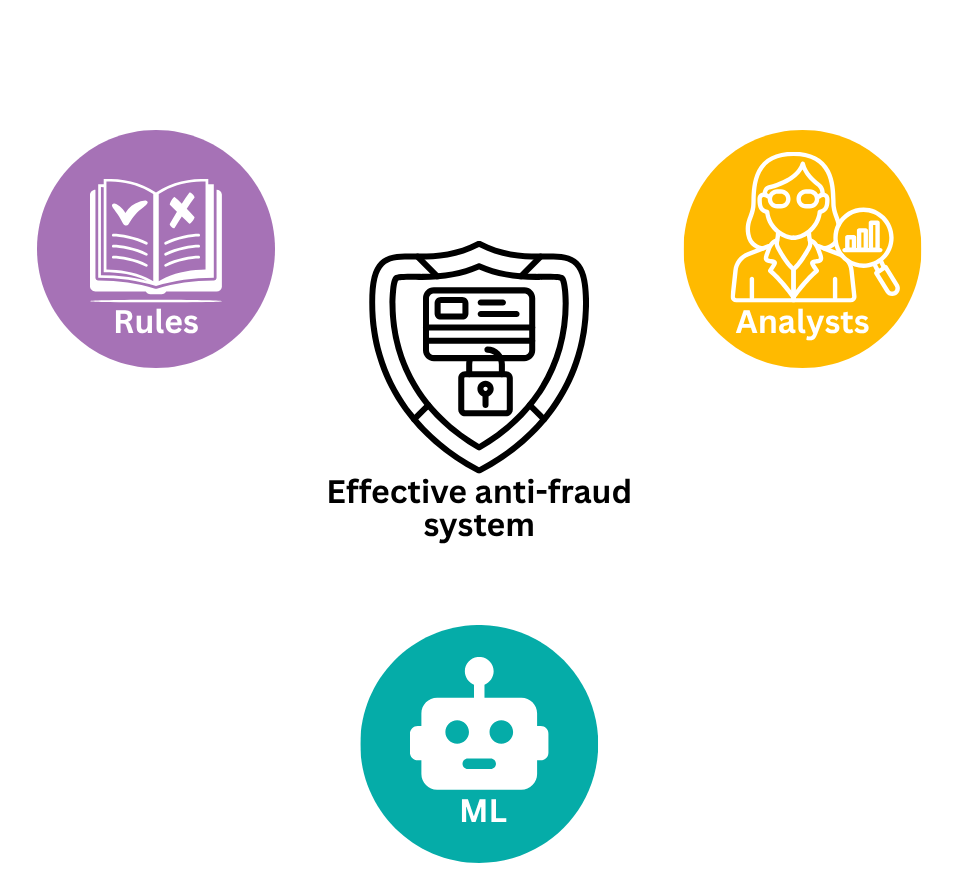
\includegraphics[width=0.50\textwidth]{fraud_system_three_pillars.png}
\caption{Effective fraud systems are built from the interaction of rules, ML, and expert analysts.}
\label{fig:three-pillars}
\end{figure}

Figure~\ref{fig:three-pillars} captures the argument in its simplest form. Rules encode explicit knowledge. ML compresses signals into scores. Analysts contribute judgment, novelty detection, and feedback. The point is to design their interaction well.

\section{Why fraud prevention becomes an architecture problem}

Fraud prevention is not a stable prediction problem. Systems combine rules, supervised models, anomaly detection, and human investigation because no single technique handles novelty, delayed labels, and operational constraints \citep{Carcillo2021, HernandezAros2024}.

\defn{\textbf{Adversarial adaptation:} Fraudsters change tactics once a defense becomes known, making detection a moving contest.}%
First, attackers adapt \citep{Bolton2002, Carcillo2021, Lunghi2023}.

\defn[0.5cm]{\textbf{Label delay:} Ground truth is often confirmed only after complaints or investigations---incomplete at decision time.}%
Second, labels are delayed and imperfect \citep{Carcillo2021, Lunghi2023}. The system acts inside the environment that later generates its own labels.

\defn[0.45cm]{\textbf{Asymmetric error costs:} False negatives cause direct loss; false positives cause friction. Not interchangeable.}%
Third, error costs are asymmetric \citep{Bolton2002, HernandezAros2024}.

\defn[0.45cm]{\textbf{Time sensitivity:} A correct decision made too late may still be operationally poor.}%
Fourth, many decisions are time-sensitive \citep{Bolton2002, Lunghi2023, Carcillo2021}. Architecture determines which cases are handled automatically and how scarce analyst attention is reserved for the ambiguous zone.

These properties explain the move toward system-centric and architecture-centric thinking \citep{Muccini2021, Lewis2021Challenges, Nazir2024}.

\section{From hidden technical debt to ML-enabled fraud systems}

\defn{\textbf{Hidden technical debt:} The real cost of production ML lies mostly outside the model: data pipelines, configuration, serving, monitoring, and glue code.}%
\citet{Sculley2015} argued that much of the real cost of ML systems lies outside the model itself. A fraud model is never the whole fraud system.

\begin{figure}[H]\centering
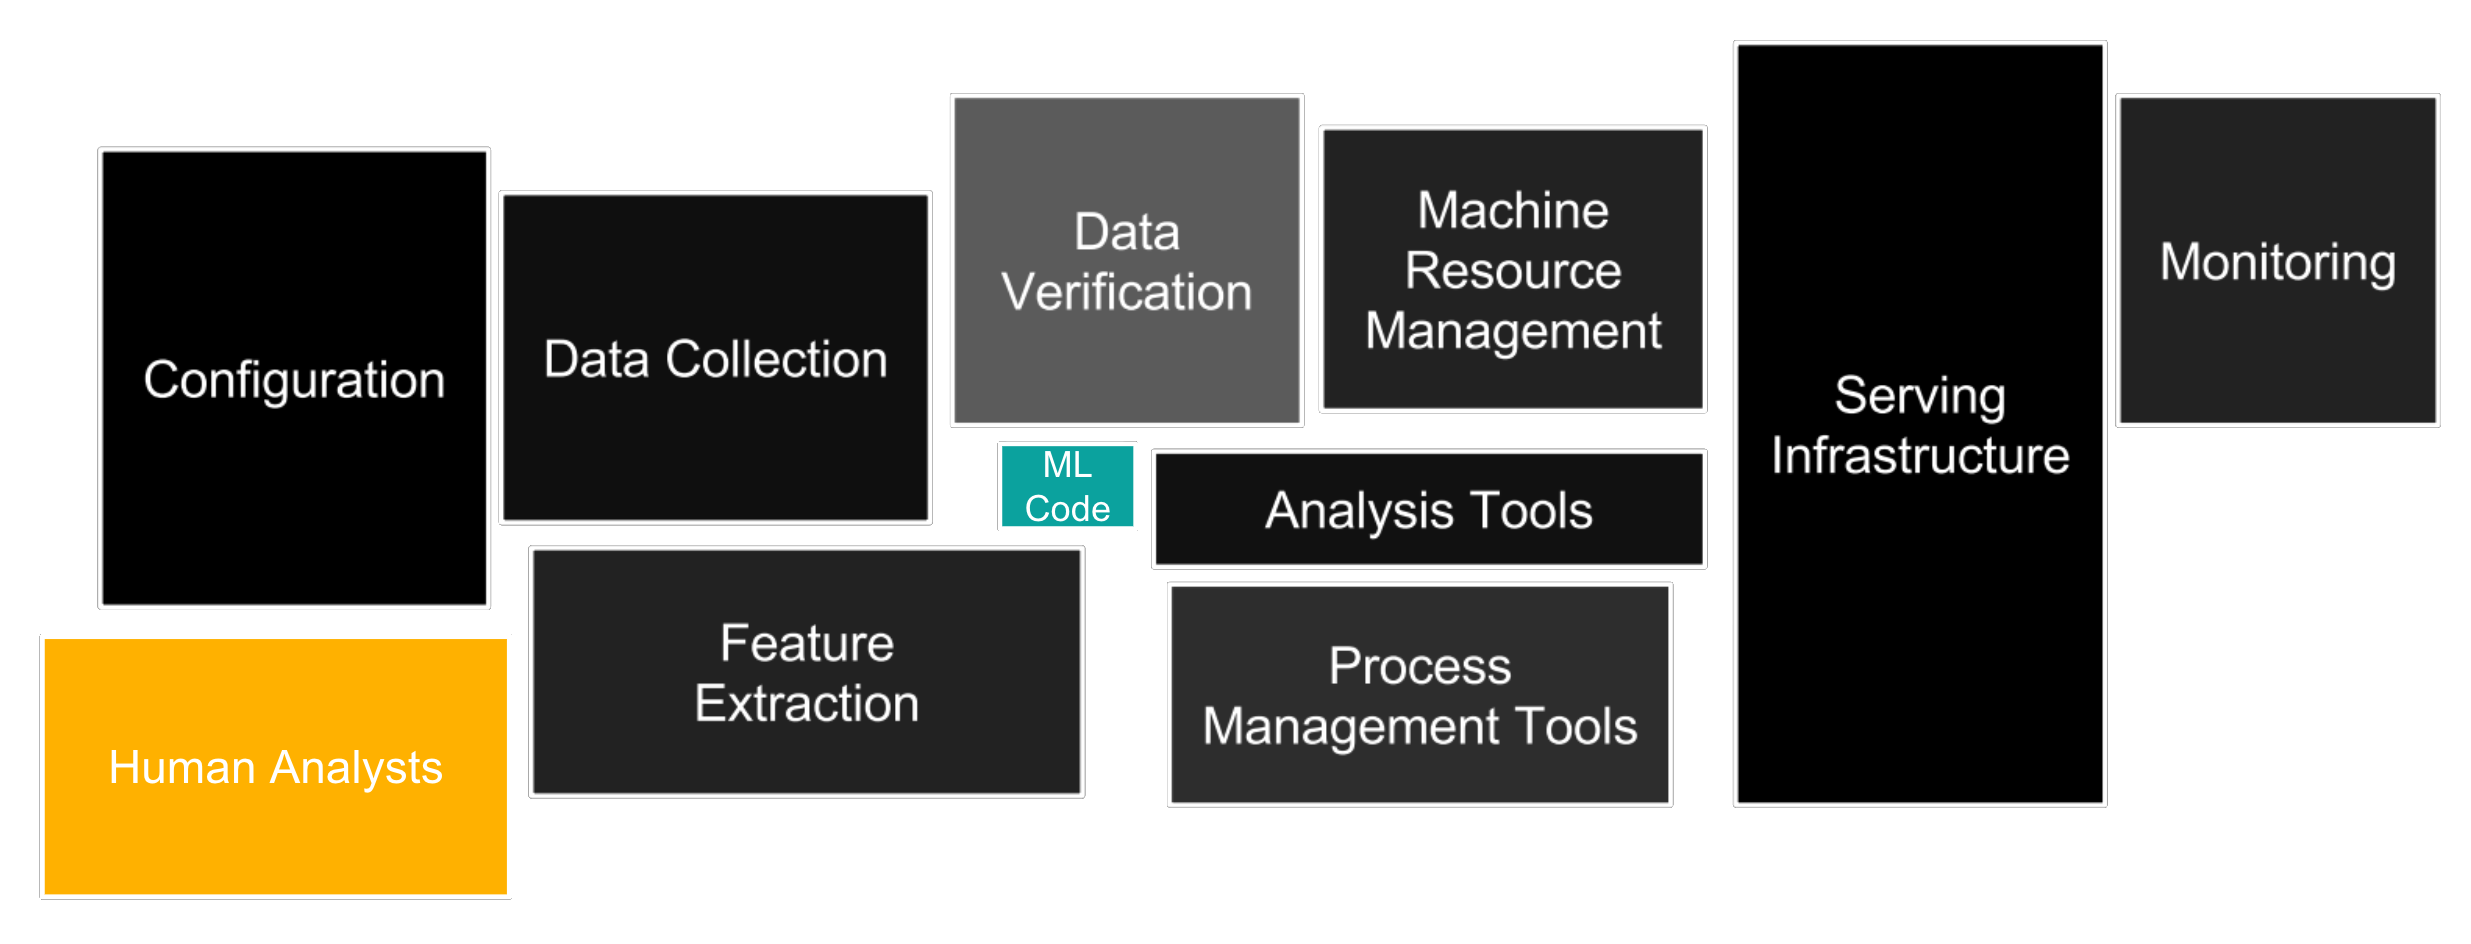
\includegraphics[width=0.75\textwidth]{system_anatomy.png}
\caption{System anatomy for fraud operations. Adapted from \citet{Sculley2015}.}
\label{fig:system-anatomy}
\end{figure}

Figure~\ref{fig:system-anatomy} places the model inside a wider environment. \citet{Lin2013} reinforce this from large-scale data-mining infrastructure.

\begin{figure}[H]\centering
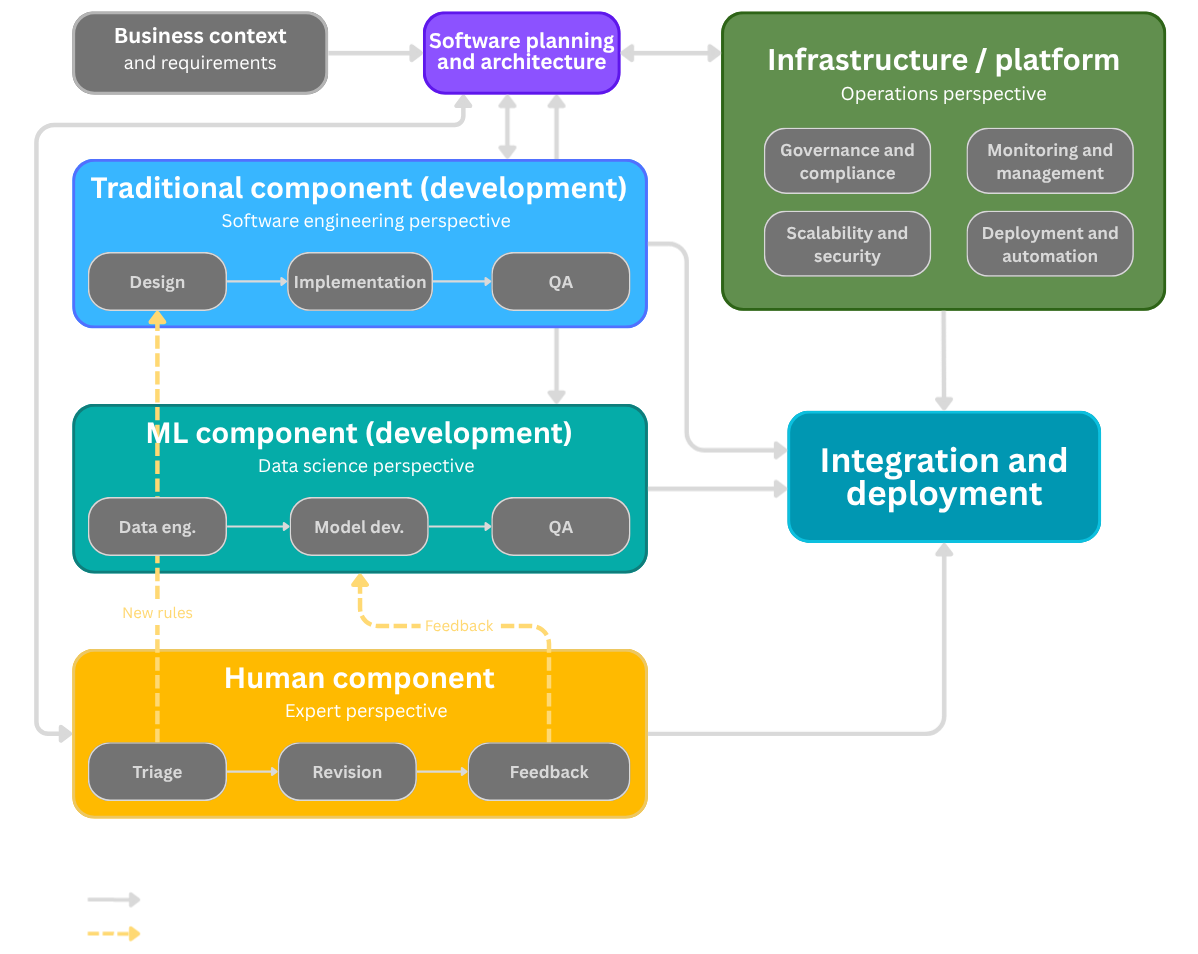
\includegraphics[width=0.75\textwidth]{ml_enabled_system_architecture.png}
\caption{Planning view. Adapted from \citet{Lewis2021Challenges}, \citet{Andersen2024}, and \citet{Kaestner2025}.}
\label{fig:planning-view}
\end{figure}

\defn{\textbf{Co-architecting:} The runtime system and model-development pipeline should be designed together.}%
\defn{\textbf{Co-versioning:} Data, features, models, evaluation artifacts, and policy thresholds should be traceable together.}%
Figure~\ref{fig:planning-view} broadens the lens to planning. \citet{Lewis2021Challenges} motivate co-architecting and co-versioning. The added human lane makes explicit what fraud operations often leave implicit.

\section{Why this article proposes a design pattern}

\defn{\textbf{Design pattern:} A reusable solution to a recurring problem. Specifies context, forces, solution, and consequences.}%
The architecture is proposed as a reusable response to a recurring class of problems.

\defn[0.55cm]{\textbf{ML architecture patterns:} Washizaki et al.\ identified 33 ML patterns. Heiland et al.\ expanded to 70.}%
\citet{Washizaki2020} documented recurring ML patterns. \citet{Heiland2023} expanded the repository. \citet{Jarvenpaa2024} focused on reusable tactics. \citet{Cruz2023} reinforced architecture rationale.

\defn{\textbf{HIL patterns:} Andersen \& Maalej catalog reusable HIL patterns spanning data prep, training, operation, monitoring, explanation.}%
\citet{Andersen2024} frame HIL as a design space with reusable patterns.

\defn{\textbf{HIL-ML family:} Active learning, interactive ML, machine teaching. Differs in \emph{how} and \emph{when} human expertise enters the loop.}%
\citet{MosqueiraRey2023} describe HIL-ML as a family of approaches.

\begin{figure}[H]\centering
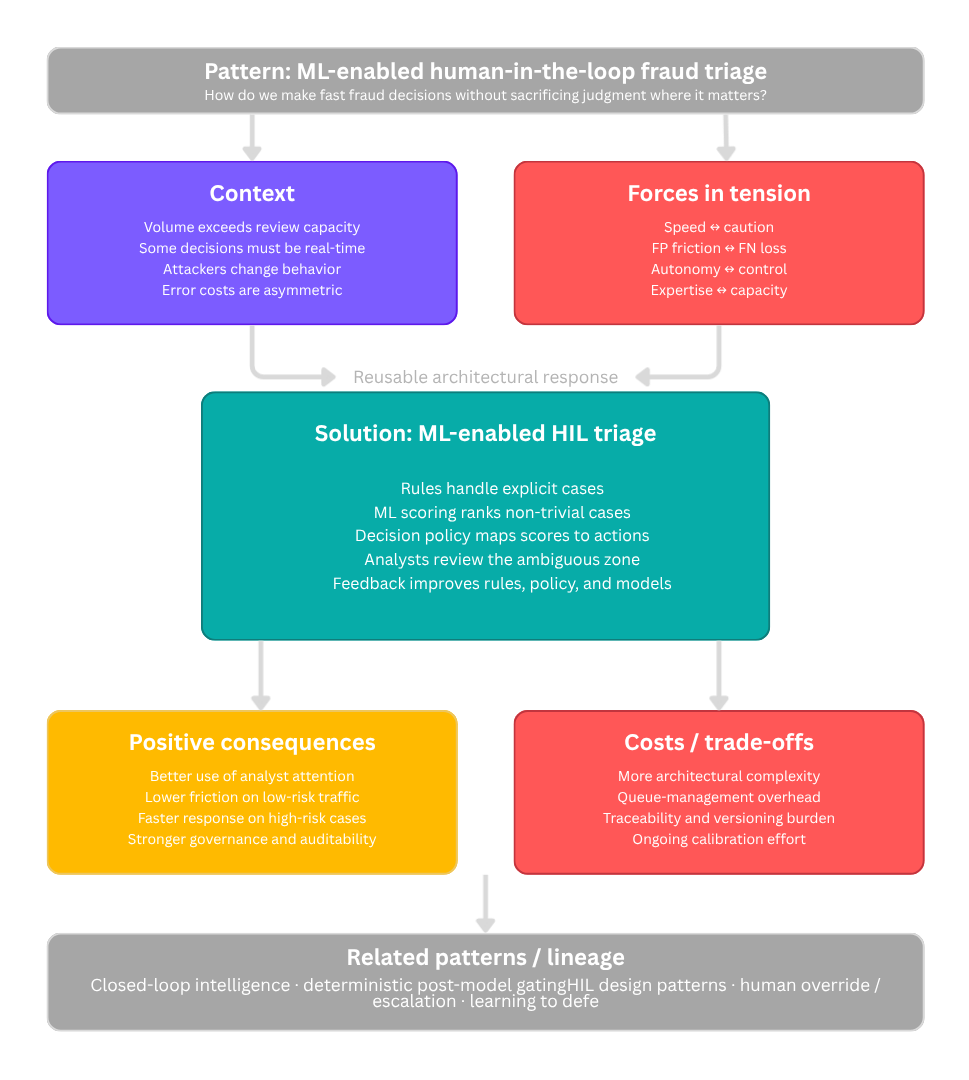
\includegraphics[width=0.65\textwidth]{pattern_context_forces_consequences.png}
\caption{Pattern framing for ML-enabled HIL fraud triage. Synthesized from \citet{Lakshmanan2020}, \citet{Andersen2024}, \citet{Heiland2023}, \citet{Cruz2023}, \citet{Jarvenpaa2024}.}
\label{fig:pattern-card}
\end{figure}

Figure~\ref{fig:pattern-card} summarizes the pattern view. Forces and consequences make trade-offs explicit, which is central to architectural reasoning \citep{Richards2025}.

\section{The anatomy of the proposed pattern}\label{sec:anatomy}

\defn{\textbf{Score $\neq$ decision:} The model produces a risk estimate. A separate policy layer translates it into action under business constraints.}%
The pattern is a series of transformations: observation to score, score to policy, policy to action.

\begin{figure}[H]\centering

\includegraphics[width=0.65\textwidth]{score_policy_action.png}
\caption{Score-to-policy-to-action pipeline.}
\label{fig:score-policy-action}
\end{figure}

The separation in Figure~\ref{fig:score-policy-action} avoids treating the score as a business decision \citep{Chen2022, Kaestner2025}.

\defn{\textbf{Learning to defer (L2D):} The system decides whether to handle a case automatically or route it to a human expert.}%

\begin{figure}[H]\centering
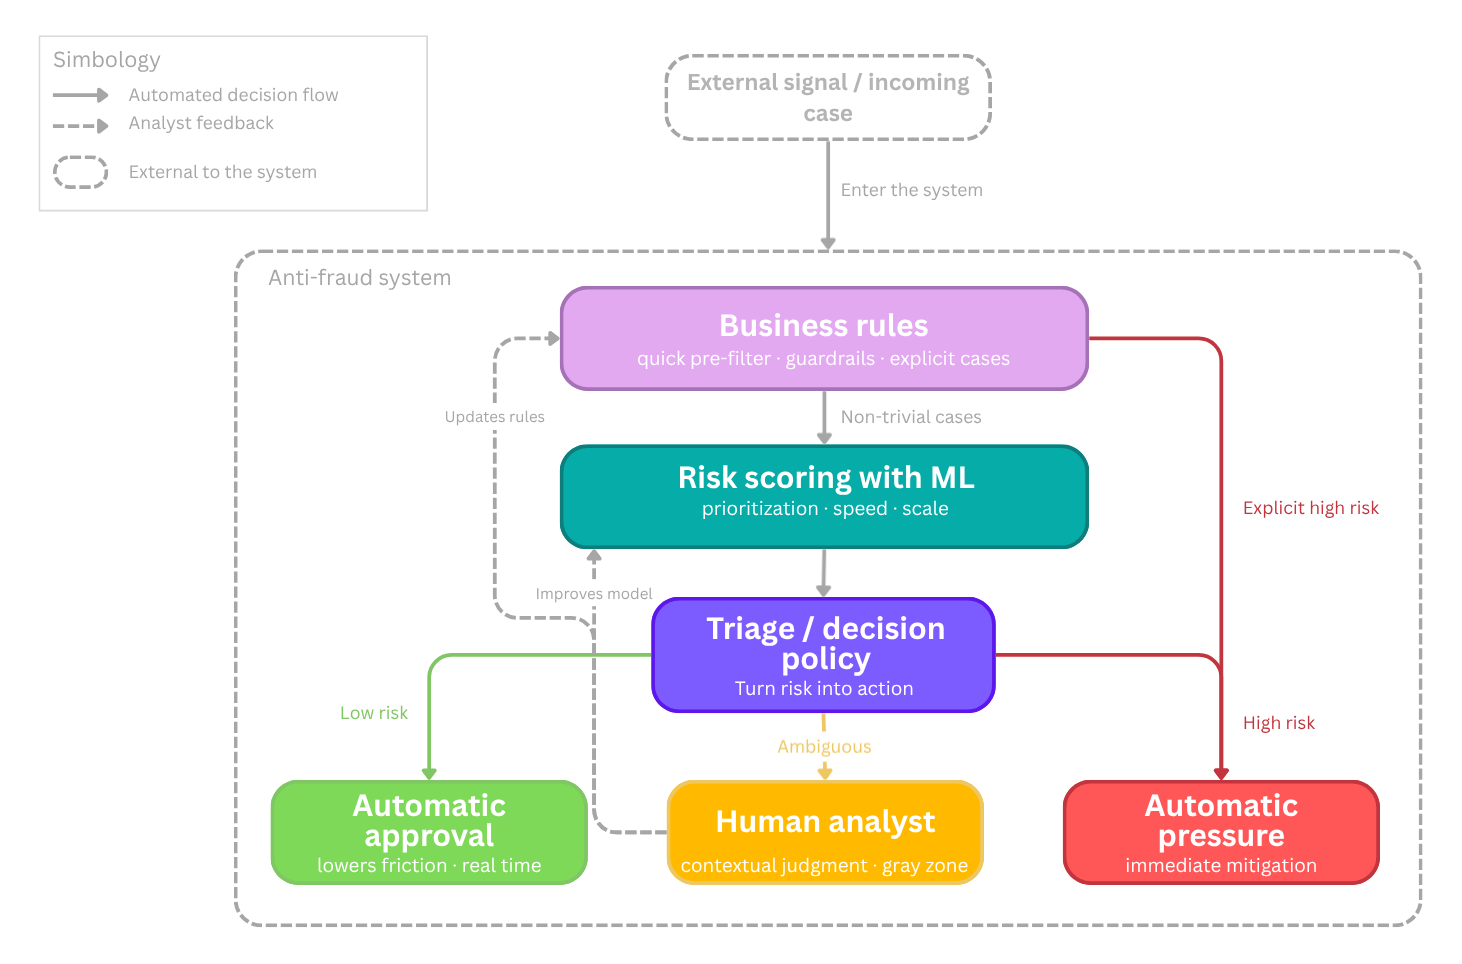
\includegraphics[width=0.75\textwidth]{hil_triage_reference_architecture.png}
\caption{Reference architecture of the ML-enabled HIL Triage pattern.}
\label{fig:reference-architecture}
\end{figure}

Figure~\ref{fig:reference-architecture} summarizes the runtime logic. This aligns with the learning-to-defer literature \citep{Alves2025}.

\section{Analysts are a runtime component, not a fallback afterthought}

\defn{\textbf{Analyst as component:} Designed workflow with structured inputs (ranked cases, reason codes) and structured outputs (decisions, feedback).}%
Analysts should be explicit runtime components.

\begin{figure}[H]\centering
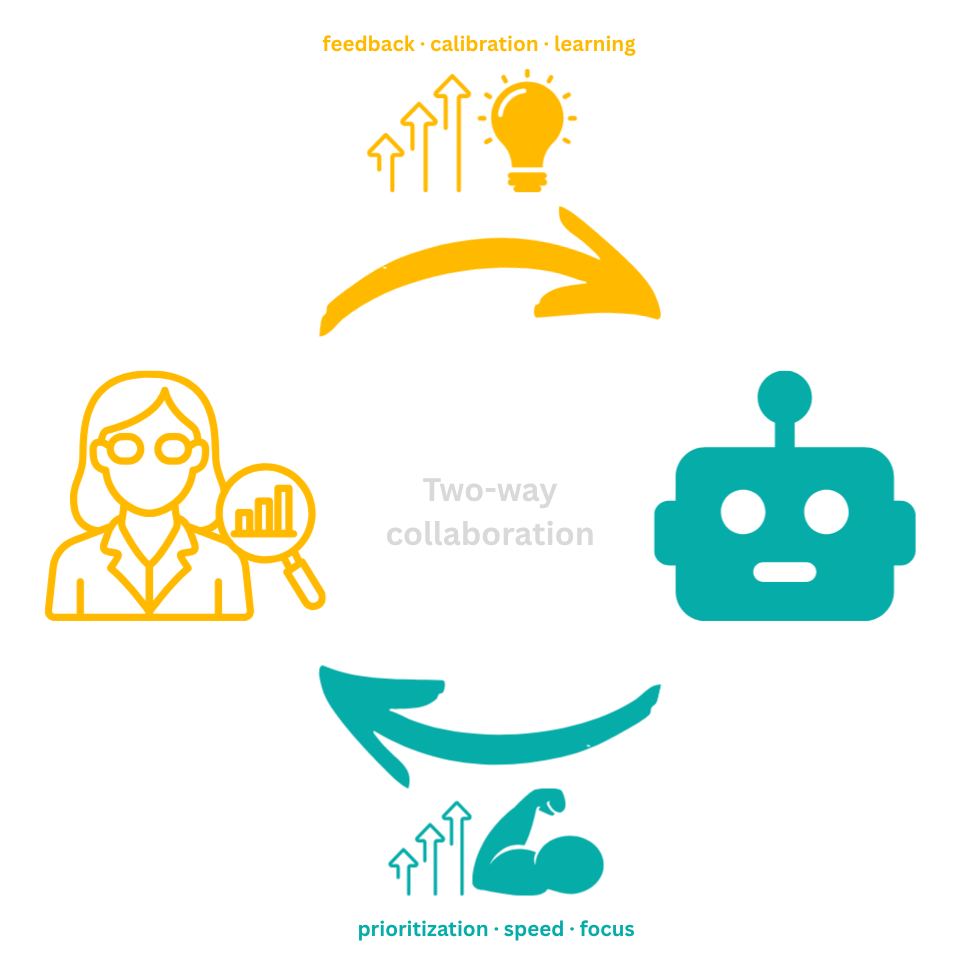
\includegraphics[width=0.45\textwidth]{bidirectional_human_ml_collaboration.png}
\caption{Bidirectional collaboration between analysts and ML.}
\label{fig:bidirectional}
\end{figure}

Figure~\ref{fig:bidirectional} shows two-way collaboration \citep{MosqueiraRey2023, Ding2023}.

\begin{figure}[H]\centering
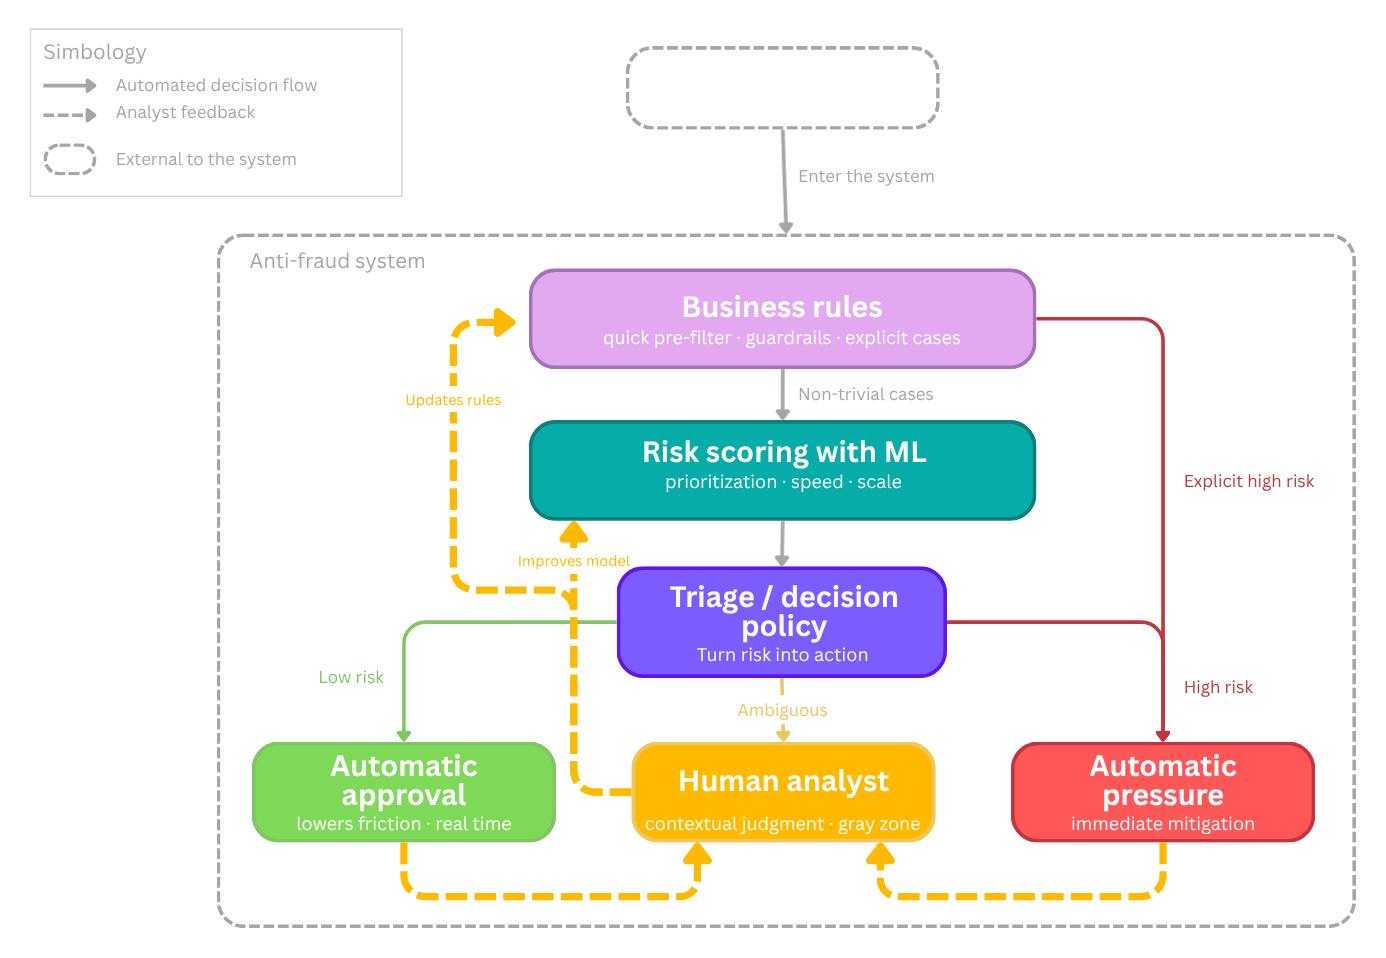
\includegraphics[width=0.75\textwidth]{hil_triage_feedback_architecture.png}
\caption{Closed-loop HIL triage with explicit feedback paths.}
\label{fig:feedback-architecture}
\end{figure}

\defn{\textbf{Feedback propagation:} Even sparse analyst annotations can improve models when propagated through a transaction graph.}%
\citet{Kadam2024} treats feedback as propagable and reusable signal.

\defn[0.65cm]{\textbf{Open-set recognition:} Detecting cases outside any known class. Human review is most valuable at the boundary of model knowledge.}%
Expert-in-the-loop approaches suggest human review is most valuable where the model faces novelty \citep{Yuan2026}.

\defn[0.68cm]{\textbf{Retrospective audit:} Review samples of automatically resolved cases to catch errors and revise routing logic.}%
Analysts should also audit automatically resolved cases \citep{Tan2026, Chen2022, Andersen2024, Kadam2024}.

\begin{figure}[H]\centering
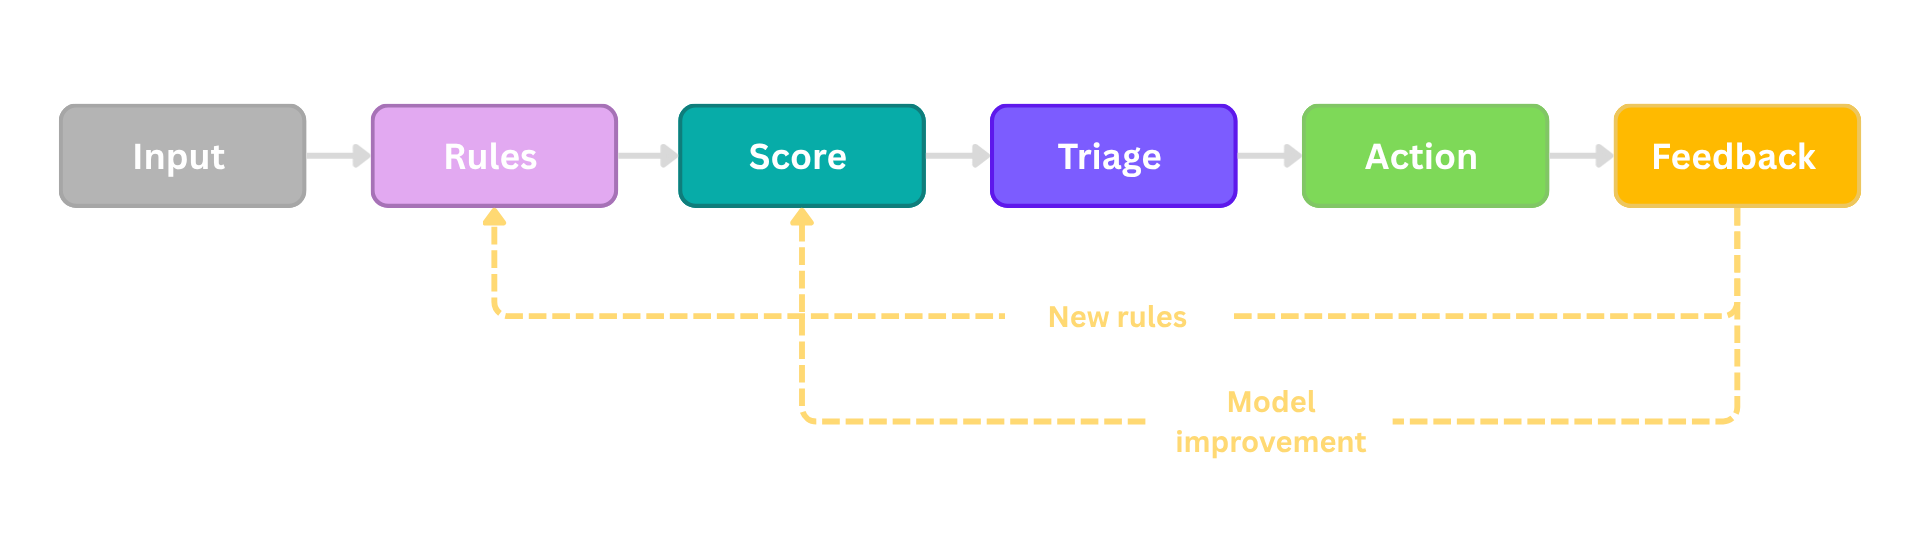
\includegraphics[width=0.75\textwidth]{operative_learning.png}
\caption{Operative learning: the pattern is a loop, not a pipeline.}
\label{fig:operative-learning}
\end{figure}

\defn{\textbf{Analyst workbench:} Ranked cases, risk bands, reason codes, SLA timers, action controls, structured feedback fields.}%

\begin{figure}[H]\centering
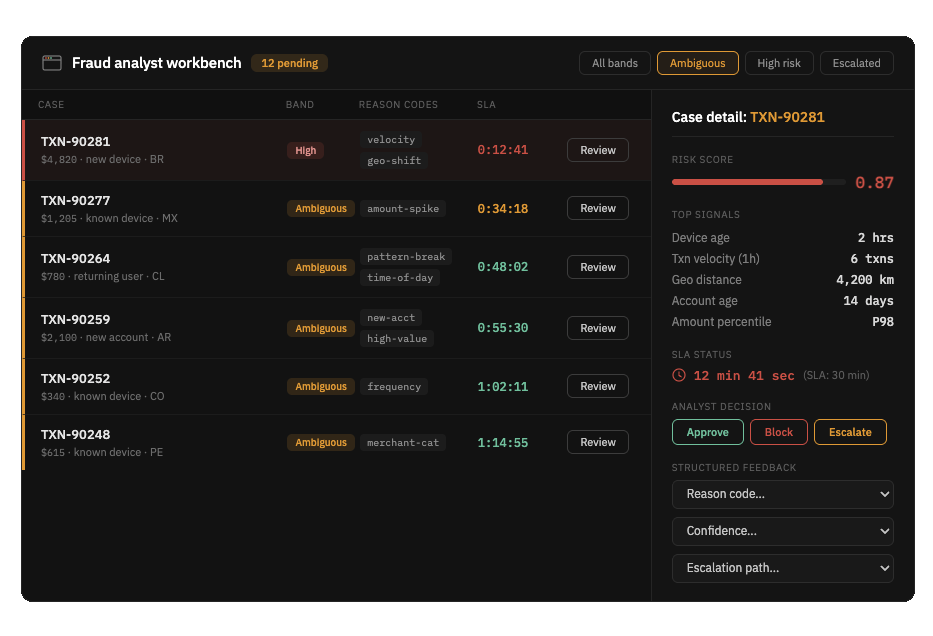
\includegraphics[width=0.75\textwidth]{analyst_queue_ui_mockup.png}
\caption{Analyst workbench. Synthesized from \citet{Jalalvand2024}, \citet{Ghadermazi2024}, \citet{Alves2025}.}
\label{fig:analyst-workbench}
\end{figure}

Figure~\ref{fig:analyst-workbench} turns the architecture into an operational review system \citep{Jalalvand2024, Ghadermazi2024, Alves2025, Amershi2019HAI, Zelvenskiy2022}.

\section{Evaluation must fit the socio-technical system}

\defn{\textbf{Four evaluation layers:} (1)~Data/input quality, (2)~model/decision quality, (3)~queue/analyst operations, (4)~runtime/platform quality.}%
Evaluation has to widen \citep{Lewis2021Challenges, Nazir2024, Dobbe2024, Salwei2022}.

\begin{figure}[H]\centering
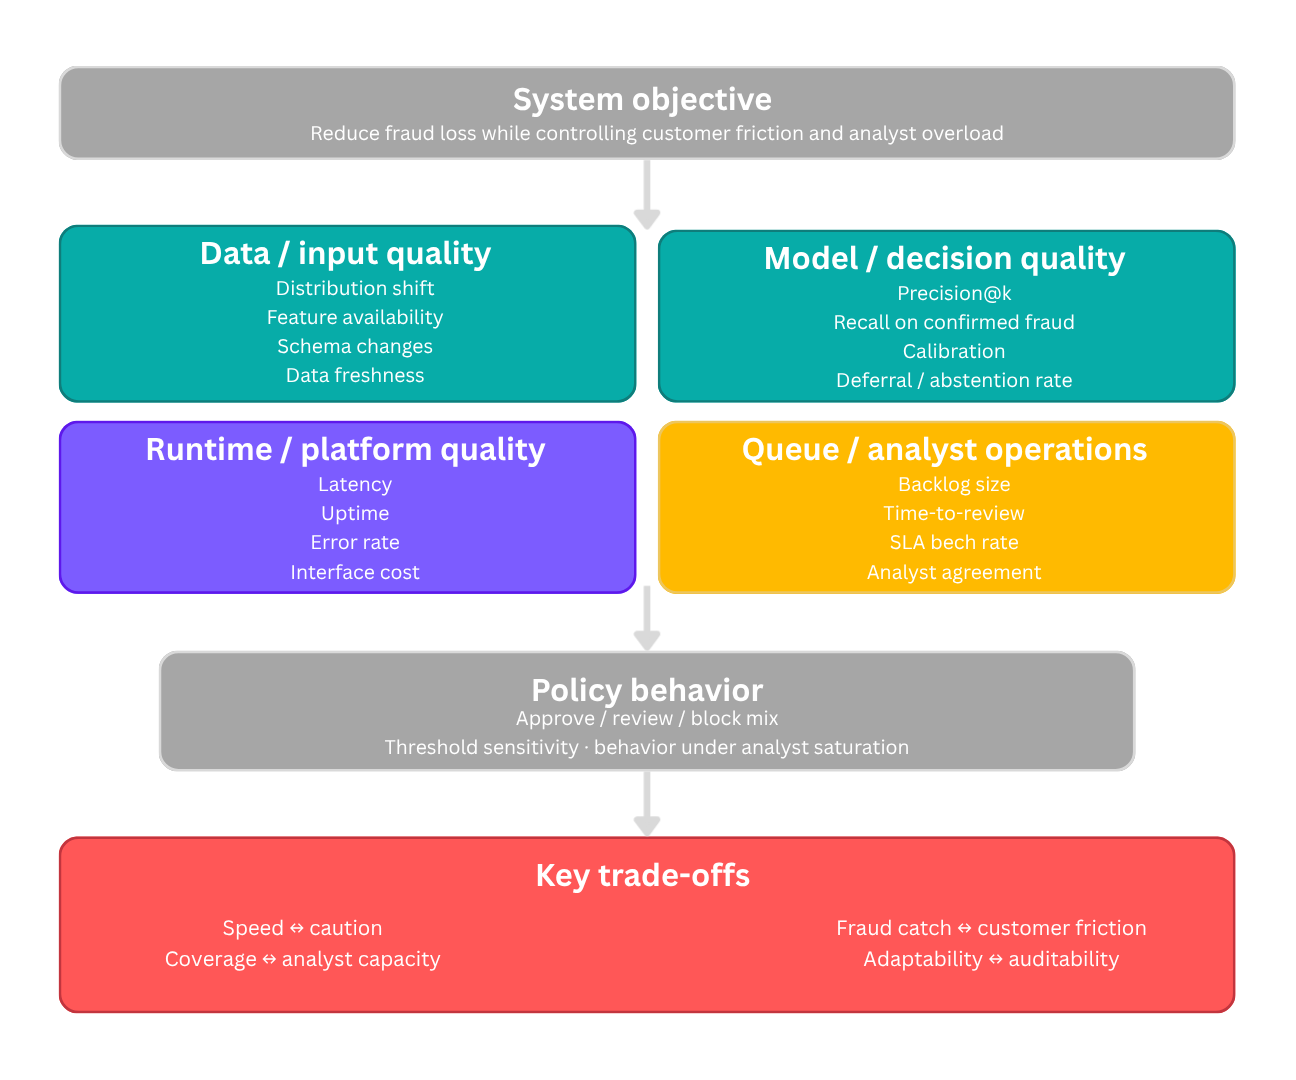
\includegraphics[width=0.75\textwidth]{metrics_and_tradeoffs_framework.png}
\caption{Metrics and trade-offs for ML-enabled HIL fraud triage.}
\label{fig:metrics-framework}
\end{figure}

\defn{\textbf{Precision@k:} Precision among the top-$k$ ranked cases. More relevant when analyst capacity is finite.}%
\defn{\textbf{Deferral rate:} Fraction of cases routed to human review. Key tuning parameter for workload.}%
Figure~\ref{fig:metrics-framework} defines a broader evaluation frame \citep{Dobbe2024, Fazelpour2025, Chen2022, Alves2025, Jalalvand2024, Ghadermazi2024, Lewis2021Challenges, Tan2026}.

\defn{\textbf{Policy behavior:} The approve/review/block split is an organizational choice, not just a model output.}%
The policy box is equally important \citep{Chen2022, Lewis2021Challenges, Kaestner2025}. The trade-off strip reflects operational frontiers \citep{Fazelpour2025, Chen2022, Richards2025}.

\section{MLOps and platform engineering are part of the argument}

\defn{\textbf{MLOps lifecycle:} Data $\to$ features $\to$ training $\to$ eval $\to$ deploy $\to$ monitor $\to$ review $\to$ feedback. Three return loops.}%
The pattern has an operational lifecycle \citep{Lewis2021Challenges, Tan2026, Kaestner2025}.

\begin{figure}[H]\centering
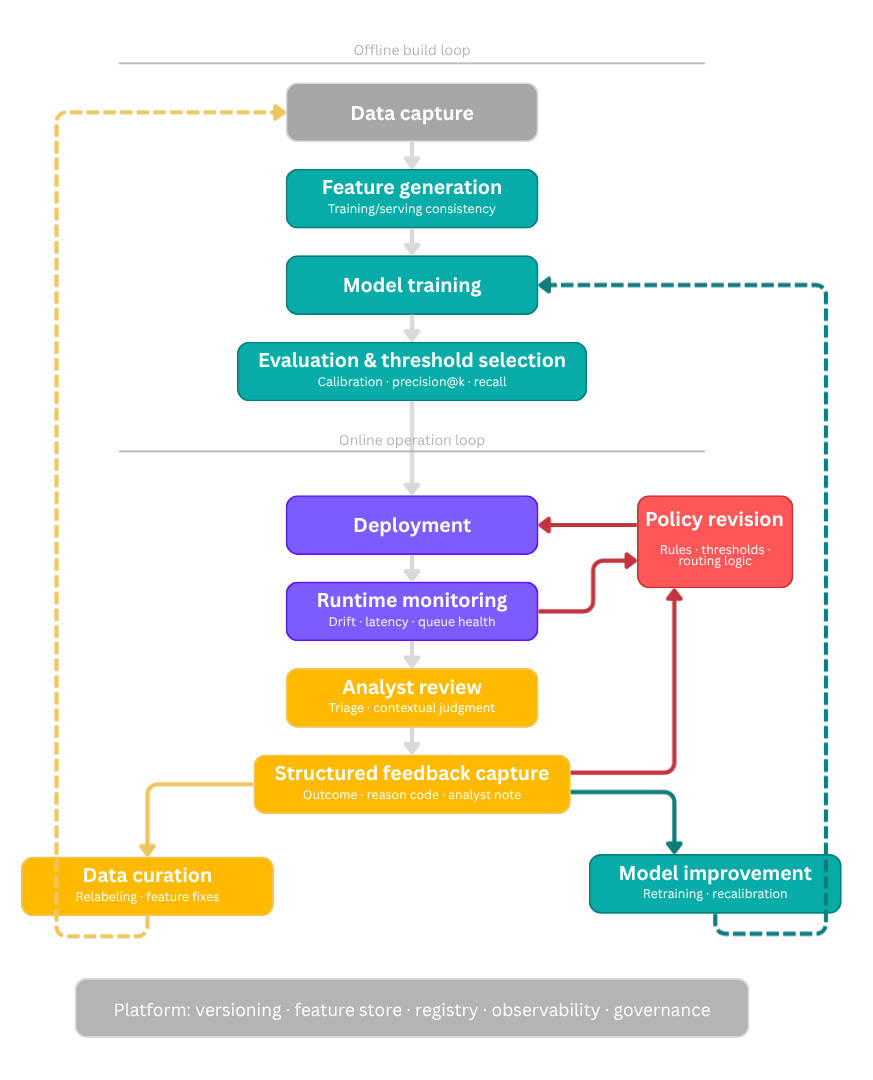
\includegraphics[width=0.75\textwidth]{mlops_feedback_lifecycle.png}
\caption{MLOps feedback lifecycle. Adapted from \citet{Lewis2021Challenges}, \citet{Tan2026}, \citet{Kadam2024}.}
\label{fig:mlops-lifecycle}
\end{figure}

\defn{\textbf{Monitorability:} First-class quality attribute. Separate monitoring for data, model, service, and queue health.}%
The side loops show why feedback should not be collapsed \citep{Lin2013, Konieczny2025, MosqueiraRey2023, Lewis2021Challenges, Lewis2021Mismatch, Kadam2024}.

\defn{\textbf{ML platform:} Versioning, feature store, model registry, observability, governance. Reduces accidental complexity.}%
Versioning, feature storage, registry services, observability, and governance are part of what makes the architecture maintainable.

\section{What the pattern improves, and what it costs}

The pattern improves analyst efficiency \citep{Jalalvand2024, Alves2025}, reduces friction \citep{Jalalvand2024, Kaestner2025}, separates inference from governance \citep{Chen2022, Lewis2021Challenges}, and makes learning explicit \citep{Andersen2024, MosqueiraRey2023}. Costs include more moving parts \citep{Lewis2021Challenges, Nazir2024}, queue monitoring \citep{Jalalvand2024, Ghadermazi2024}, versioned decision logic \citep{Lewis2021Challenges, Cruz2023}, and cross-team coordination \citep{Nazir2024, Richards2025}.

\subsection{Anti-patterns worth naming}

\defn{\textbf{Anti-pattern --- Score = policy:} Raw scores trigger actions; governance becomes opaque.}%
\textbf{Letting the score become policy} \citep{Lewis2021Challenges, Washizaki2020}. Remedy: Section~\ref{sec:anatomy} \citep{Washizaki2020, Kaestner2025}.

\defn{\textbf{Anti-pattern --- Unstructured HIL:} Free-text-only review generates cost but no reusable signal.}%
\textbf{Treating analysts as unstructured exception handling} \citep{MosqueiraRey2023, Andersen2024}.

\textbf{Building the model while leaving operations underspecified} \citep{Jalalvand2024, Lewis2021Challenges, Nazir2024}.

\textbf{Ignoring monitorability until something breaks} \citep{Lewis2021Challenges, Jalalvand2024}.

\defn{\textbf{Anti-pattern --- Pipeline jungle:} Feature joins, rule engines, risk services accumulate without platform discipline.}%
\textbf{Glue code and pipeline jungles} \citep{Washizaki2020, Lewis2021Challenges, Kaestner2025}. These anti-patterns define the pattern's limits \citep{Richards2025, Cruz2023}.

\section{Why this matters for a new, but important field}

ML-enabled software architecture is still young \citep{Muccini2021, Nazir2024}. Human participation is itself a design space \citep{MosqueiraRey2023, Andersen2024}. Fraud makes the socio-technical nature of ML visible \citep{Dobbe2024, Salwei2022, Kaestner2025}. This pattern adds one concrete example to that growing field \citep{Washizaki2020, Andersen2024, Kaestner2025, Richards2025}.

\section{Open questions}

One concerns \textbf{policy optimization}. Another concerns \textbf{feedback quality} \citep{Alves2025, Yuan2026}. A third concerns \textbf{architecture evaluation} \citep{Cruz2023, Nazir2024, Jalalvand2024, Chen2022, Lunghi2023}. A fourth concerns \textbf{platform productization} \citep{Lin2013, Tan2026}.

\defn{\textbf{LLM integration:} How to add NL case summarization and conversational investigation without undermining structured feedback and auditability.}%
A fifth concerns \textbf{LLMs in the analyst workflow}: how to integrate case summarization, reasoning traces, and explanation interfaces without weakening governance \citep{Tan2026}.

\section{Conclusion}

Fraud prevention should be designed as an ML-enabled socio-technical architecture. Use rules where explicit knowledge exists. Use ML where prioritization creates scale. Use analysts where context and judgment matter. Keep score separate from policy. Capture feedback in structured form. Design the platform so the system can be observed, revised, and improved.

This combination of rules, scoring, policy, analyst review, and closed-loop learning deserves to be treated as a reusable architectural response for a high-stakes domain.

\bibliography{references}
\end{document}